\section{Metodología de desarrollo}

Para el desarrollo se software se utiliza un modelo de entrega por etapas. Este modelo, como se observa en la figura \ref{fig:modelo_etapas}, realiza las primeras etapas de forma secuencial y permite diseñar e implementar los componentes del proyecto por separado. Seguir este modelo permite entregar partes del proyecto y tener visibilidad del progreso. 

\begin{figure}[htbp]
	\centering
	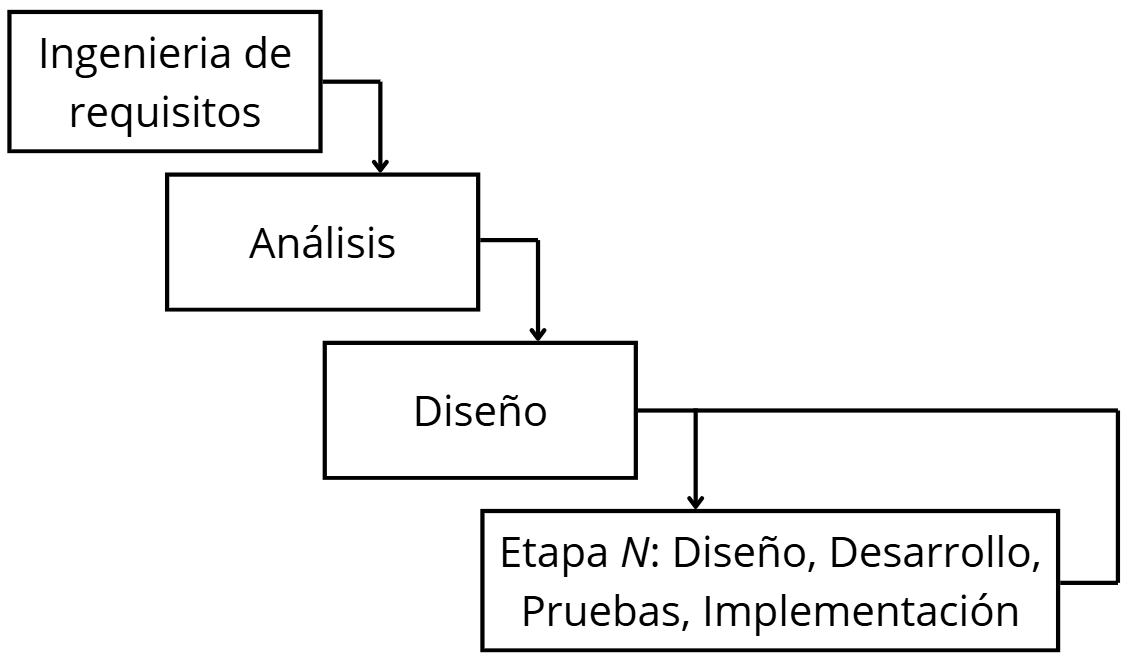
\includegraphics[width=0.75\linewidth]{img/modelo_etapas.png}
	\caption{Representación grafica del modelo de entrega por etapas para el desarrollo del software}
	\label{fig:modelo_etapas}
\end{figure}

Estas son algunas de las razones por la cual se opta por este modelo:

\begin{itemize}
	\item El tamaño del equipo de desarrollo es reducido: Al tener un numero de integrantes reducido, resulta inviable desarrollar múltiples componentes de forma paralela. 
	
	\item No existe un cliente: El desarrollo de este producto de software es unicamente un medio para el proceso experimental.
	
	\item No es un producto comercial: No se planea monetizar dado que no existe un cliente. Por lo que en la ingeniería de requisitos se consideran los necesarios propuestos por el equipo de investigación para satisfacer las necesidades tecnológicas.

	\item No hay procesos iterativos: Al no tener cliente no es necesario tener una validación externa, ni cambios significativos en los requerimientos del software. 
\end{itemize}